%%%%%%%%%%%%%%%%%%%%%%%%%%%%%%%%%%%%%%%%%%%%
%%% OCCULTISM
%%%%%%%%%%%%%%%%%%%%%%%%%%%%%%%%%%%%%%%%%%%%

\newpage


\mysection{Occultism}{marvels-occultism}

    \flavor{
        Where's the game in life, behind the game behind the game... \Tilde Public Enemy
    }


In order to practice the sacred and profane rites and rituals of Occultism, you must possess \mylink{Cunning}{mystic-virtue-cunning}, meaning your Fate is now bound to the Wheel.  Your position on the Wheel, as well as the presence of a Familiar or a Coven will increase your Cunning as follows:

Cunning is required to practice the observances and ceremonies that make up Occultism.   

  \mytable{X X}{}
  {
    Wheel: Crown & +3 \\
    Wheel: Gibbous & +2 \\
    Wheel: Wax Quotidian & +1 \\
    Coven & +1 each member \\
    Familiar & +1 if present \\
  }  

  For some powerful occult rites, you may need to move "[num] Widdershins" before you can attempt the ritual again. A full Widdershins means you must make [num] transit(s) of the Wheel before you can cast the ritual again. For example, if you were at Crown, you must travel to Waning Gibbous, then Waning Quotidian, etc. all the way back around to Crown before you can try again (meaning you will need to play multiple Sessions).


Occultism must be practiced on \mylink{Unhallowed Earth}{occultism-unhallowed-earth}.


\cbreak


\OCCULT[
  Name=Barghest,
  Link=occultism-barghest,
  Success=10+,
  Cost=66\AG (plus see below)
]

You summon a spectral black dog (a harbinger of death and misfortune) to torment a single person for [Cunning] days.  You must whisper the birth name of the victim to the spectre; upon hearing it, the black dog will seek the victim out, traveling up to [Cunning]x100km a night to find them.  The barghest can only travel at night, and disappears at the first light of the rising sun.  The dog can see invisible or hidden creatures and will unerringly find the target provided they are within distance of the casting of the ritual.

Once found, the barghest will appear to the victim once every night.  The victim is permitted a Save vs Doom when they see the Barghest; if they fail, they suffer the curse of the Barghest until it appears again at sunset.  Pooka are immune to Barghests, and if the victim is in a Band with the Pooka, they get two Saves.

If the victim fails their save, they suffer the following maledictions:
- they automatically "take a 1" on Luck checks
- they can't heal Grit
- all \RO and \RB tests suffer a -4 penalty (excluding their Save vs Doom against the Barghest the following night)

The ritual requires a dog (your familiar is fine); an item belonging to the victim; and 66\AG in supplies.  No harm comes to the dog, but the spectral figure will resemble him or her if examined closely

\cbreak

\OCCULT[
  Name=Bind Familiar,
  Link=occultism-bind-familiar,
  Success=5+,
  Cost=666\FE
]

Your familiar is a supernatural creature bound to your soul.  They can be summoned and dismissed at will: they'll appear from a shadow (cat) or sewer grate (rat) or fly in through a window (raven), and they'll leave roughly the same way.  Familiars are Unhallowed, and grant you +1 Cunning if they're with you when you practice Occultism.  

The strength of your familiar depends on the number of [Cunning] you invest when you summon them.  They can be sent on missions up to [Cunning]km away. You can see what they see and hear what they hear for as long as you Concentrate. You also can remember things your familiar remembers (so you could send them on a spying mission and later "remember" what they saw). You can cast Charms through your familiar if you desire.

If your familiar is Close or Nearby, you can communicate verbally with them, though you cannot use words greater than 1 syllable.  You communicate in a language all your own that no one else understands.  They can follow simple instructions ("get the key on the desk", "chew through these ropes", "spy on that man") but not more complex ones ("pick the lock").  Your familiar can't talk.

Familiars have [Cunning] Health.  If you have the Mystic Virtue: Aura (see core rules), you can shield them with your Mojo the same way you shield yourself, but you can roll your Mojo as many times as you want (while it isn't exhausted, anyway) to protect them.  If they're attacked and they survive, they immediately dismiss themselves and won't return for the rest of the Session. If your Familiar dies, you must travel Widdershins before you can summon another.  

Familiars are themselves immune to spells from the Mind paradigm, but if a Mind spell is cast on them you need to Save or be affected as if the spell targeted you.

Finally, you can place a Malison on your familiar (see the ritual below).  In the event of your death, the familiar will stay with your body until someone attempts to disturb your corpse.  At that point, it will deliver the malison etched upon its skin, and dismiss itself for good.

When you summon your familiar, roll below (or discuss with the Arbiter if you want to choose), or make something up.  You can only have 1 familiar at a time.



\myhighlight{Familiars}{occultism-familiars}

  \mytable{l X}{
    \thead{d6} & \thead{Familiar}\\
  }{
    1 & Cat \\
    2 & Dog \\
    3 & Rat \\
    4 & Toad \\
    5 & Raven \\
    6 & Exotic (roll below) \\
  }  

  \mytable{l X}{
    \thead{d6} & \thead{Familiar}\\
  }{
    1 & The severed hands of a tomb robber  \\
    2 &  A floating piece of quartz \\
    3 & A 9-segmented colored cube that turns constantly  \\
    4 & A button-eyed doll made of rags and straw \\
    5 &  A tiny deformed homonculous resembling you \\
    6 & A hyper-intelligent slime \\
  }  

  \begin{center}
  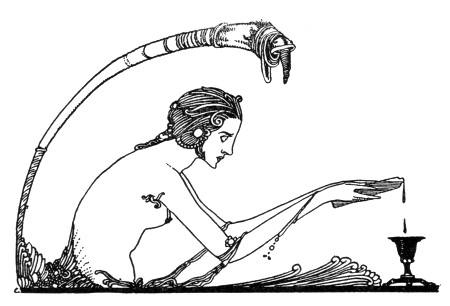
\includegraphics[scale=.5]{Occult_1}
  \end{center}


\OCCULT[
  Name=Create Juju,
  Link=occultism-create-juju,
  Success=varies,
  Cost=varies
]


Juju are minor magical items created by witches using their Mojo.  The Juju must be placed on an item OK'd by the Arbiter and should be something "special", like:

\mybullet {
  \item A carved branch of a tree that only grows in the cold stone ruins of Carcosa
  \item 3 jeweled eggs stolen from a Roc's nest when the Eye of Tartarus is full
  \item The carved fingerbones of St. Sacrastine, which reside in the sacristy of the Temple of Gomorrah in Lankhmar
  \item etc.
}

Juju can do pretty much anything you and the Arbiter agree on, but here are some ground rules for what it \mybold{cannot} do:

\mybullet {
  \item It cannot be used to deal direct damage, or be an item that causes damage directly (knives, swords, etc)
  \item It cannot be used to create a \DCUP or \DCDOWN effect
  \item It cannot duplicate the effect of any Wizardry, Liturgy, or Sacrament
  \item It cannot provide more than +4 to a specific \RO or \RB attempt
}

Each piece of Juju must have a \mylink{Witch Mark}{occultism-witch-mark} on it for every unique power that it has (at the Arbiter's discretion).

\mybold{Examples}

\ed{A few of these are from Chris McDowall's \href{https://www.bastionland.com/2009/07/100-interesting-magic-items-first-half.html}{\mybold{Bastionland}}}

\mybold{Trivial "Bush" Juju: 7 Cunning; 666\FE}

\mybullet {
    \item \mybold{Coin Beetle:} A normal looking coin. However, at night it comes to life and eats one other coin it can find, before disguising itself as a coin once again.
    \item \mybold{Frog Box:} If this box is left open near to a frog it will be compelled to hop in and sit there happily. The frog will stay in the box without needing food, air or water, until instructed to hop out.
    \item \mybold{Kingsblood Weed:} Boiling this weed produces tea that will taste delicious to anyone of royal blood but foul to anyone that isn't
    \item \mybold{Lucky Rabbit's Foot:}  Gives you a +1 on any \RO or \RB attempt that uses \DEX or Talent
}


\mybold{Minor "Sacred" Juju: 9 Cunning; 666\AG}

\mybullet {
    \item  \mybold{Dogpack Tooth:} If this tooth is pressed into someone's gums it will take root and allow the owner to speak with dogs and wolves.
    \item \mybold{Fiery Ring:} If a container of food or liquid is held in the hand bearing this ring it will slowly heat up. Within a minute it will be boiling, but the container will still be safe to hold.
    \item \mybold{Magic Mirror:}  Allows you to \mylink{Descry}{occultism-descry}
    \item \mybold{Cornicello:} Gives you +2 on your Saves vs. Doom
}


\mybold{Major "Black Magic" Juju; 11 Cunning; 666\AU}

\mybullet {
    \item \mybold{Crystal Ship:} This miniature ship is beautifully crafted and valuable, but if it is ever taken on board a ship that ship will sink before its voyage is completed.
    \item \mybold{Money Belt:} Any amount of money may be pressed into a small slot on the front of this belt.  The money enters Hammerspace. The money can be retrieved by tapping it three times and announcing how much is required. This will even cause larger coins to be converted into change for specific amounts.
    \item \mybold{Bezoar Necklace:}  When worn around the throat, grants +3 to Saves vs. Toxins.
    \item \mybold{Phylactery:} A receptacle appropriate for the ritual of Lichdom.
}

  \begin{center}
  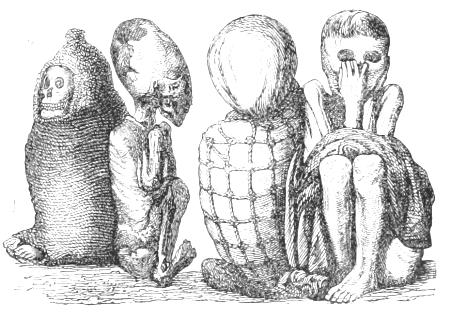
\includegraphics[scale=.5]{Fetish_or_Juju}
  \end{center}

\mybold{Supreme "Devil's" Juju; 13 Cunning; 6{,}666\AU}

\mybullet {
    \item \mybold{Ether Flute:} Playing this flute causes any Incorporeal Monster to freeze, mesmerized, so long as the user continues to play.
    \item \mybold{Golden Mule:} A tiny golden statue of a mule. Anyone carrying this doubles the number of Significant Items they can carry
    \item \mybold{Master's Ring:} This ring causes a faint tingling sensation whenever one of the wearer's employees, servants or hirelings is planning to betray them in some way.
    \item \mybold{The Displacement Doll:} Anyone attempting any Mind spell on the possessor of the Displacement Doll kind will affect only the mind of the doll. If they try to read her mind, they will read the mind of a woman trapped in a dark leather chamber, bouncing around on the body of a giant. If they try to charm her they will successfully charm the doll. 
    \item \mybold{Shrunken Head:}  Wearing the Shrunken Head on your belt gives you a +4 modifier on your \DEATH rolls
}

\OCCULT[
  Name=Damning,
  Link=occultism-damning,
  Success=9,
  Cost=666\AG
]

When you perform this ritual on a Mortal corpse no more than 7 days dead (by the law of \TheAuthority), you prevent them from departing the Isle of the Dead.  The soul is trapped in Hell permanently (though their spirit can still be lead back to the Mortal plane through \mylink{Katabasis}{occultism-katabasis}.  The corpse is consumed when this ritual is performed.


\OCCULT[
  Name=Descry,
  Link=occultism-descry,
  Success=3+,
  Cost=See below
]

You can see events transpiring within [Cunning]x100km of you by gazing into a silver bowl, censer, crystal ball, mirror, or other mystical item.  You only need to describe what you want to see and it will appear, but the vision is misty and it's hard to make out details.  You can't see things that you might not normally be able to see, so if you said you wanted to "see the body of Sir Tremalane on the northern battlefield", and the body was invisible, you might only see a bare patch of ground.  

The scrying doesn't have to only show events of the present; you can look up to [Cunning] centuries into the past.  You'd have to have a rough idea of what you'd want to see - "show me the temples of Syrinx before they were cast down" would work, but "show me the secret entrance to the Caverns of Chaos" wouldn't.  The more detailed the description of what you want to see, the better you see it.

Scrying requires that the silver bowl, censer, crystal ball be a \mylink{Minor, Major, or Greater Juju}{occultism-create-juju}.  Major Juju adds 100km and 100 years; Greater Juju adds 1,000km and 1,000 years.

  \begin{center}
  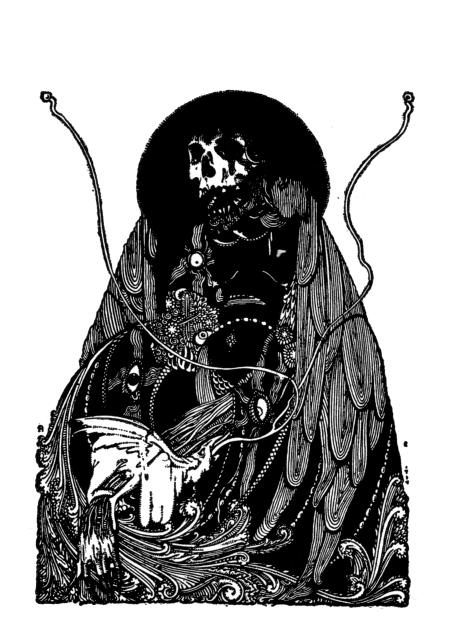
\includegraphics[scale=.5]{Occult_2}
  \end{center}



\OCCULT[
  Name=Geas,
  Link=occultism-geas,
  Success=12,
  Cost=666\AU
]

\ed{From \mybold{Places Dark \& Deep}, by the author of the blog \href{https://permacrandam.blogspot.com/}{Permanent Cranial Damage}}

You ensorcel someone with a Geas, a terrible malison that enforces an inescapable command. The command can be long and difficult, like "kill Razor the Monk" or "complete the seven-fold pilgrimage" or "bring me the Globe of the Wonder-Working King from the hoard of the Caliph Vathek" or "go away". The victim must win a \RB : \FOC contest against you.  From then on, any day that is not spent fulfilling the Geas will have one of the following effects (roll each day):

\mynumlist {
  \item Inflicted with a Greater Curse (roll on the Curse table, re-roll any duplicates)
  \item Inflicted with a Disease (roll on the Diseases table, re-roll any duplicates)
  \item Inflicted with a Wound (roll on the Wounds table as if the target had been brought to 0 Flesh)
  \item Roll a d6: 1-3 all Tangible Stats \DCDOWN; 4-6 all Intangible Stats \DCDOWN
  \item Inability to "heal" in any way - you gain absolutely no benefits from resting
  \item Roll again - the result of the roll is inflicted on the target's loved one / parent / child / friend / etc. instead.  If the target loves nothing, the Arbiter gets to choose
}

The effect lasts until sundown; provided the subject of the Geas is "back on track", the effect ends - otherwise, roll again.

The Geas must be doable, even if it is way above the means and possibility of the victim.  Should it become impossible (following the examples above: if Razor should die in other ways, or one of the Seven Shrines be destroyed, or the Orb suddenly explode and release the 1001 demons bound inside), then the Geas is lifted.  Should you or the victim die, the Geas remains in effect, even if you are brought back from the dead or turned into undead. This spell cannot be cast on someone more than once in their lifetime.

On the upside, the Geas can empower its subject (at the Arbiter's discretion) to help them complete their task.  For example, if Razor the Monk has taken up with the King of the Merfolk, the subject of the Geas might discover they can now breathe underwater.

The target of the Geas needs to be conscious and near you when you invoke the ritual.

\OCCULT[
  Name=Haunt,
  Link=occultism-haunt,
  Success=3+,
  Cost=666\FE
]

\ed{From \mybold{Places Dark \& Deep}, by the author of the blog \href{https://permacrandam.blogspot.com/}{Permanent Cranial Damage}}

You summon [Cunning] poltergeists to haunt an Unhallowed place up to [Cunning]km away.  The poltergeists will do their best to harass and torment any Mortals who enter their domain. They can't talk and are insubstantial, but you can direct them to laugh insanely, become visible as ghostly menaces, howl discordantly, and cause telekinetic mischief, which may include the hurling of heavy or sharp objects.

\OCCULT[
  Name=Hekaphage,
  Link=occultism-hekaphage,
  Success=4+,
  Cost=varies
]

You can destroy a malison by feeding it to a Hekaphage: ethereal creatures that eat magic and Curses.  

\mybullet{
    \item a Lesser Curse requires 4 [Cunning]
    \item a Greater Curse requires 8 [Cunning]
}

Summoning a Hekaphage costs no coin (only Unhallowed Earth), but you can spend up to [Cunning]x100 coins in materials if you would like to convert coin to Glory.

\cbreak

  \begin{center}
  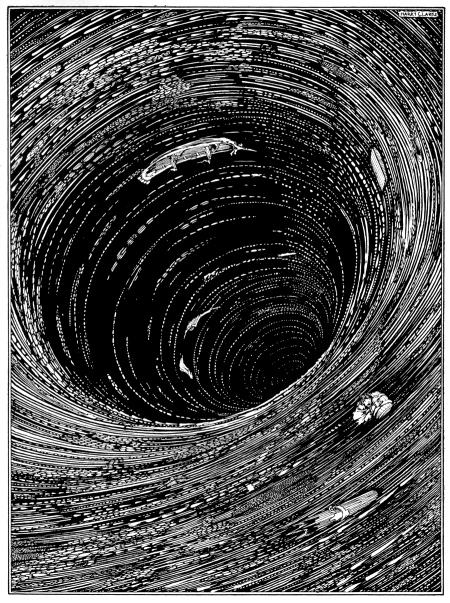
\includegraphics[scale=.5]{Occult_3}
  \end{center}





\OCCULT[
  Name=Katabasis,
  Link=occultism-katabasis,
  Success=15,
  Cost=6{,}666\AU
]

\ed{Idea for the Isle of the Dead comes from Arnold Kemp's \href{https://goblinpunch.blogspot.com/2015/04/the-isles-of-dead.html}{"Goblin Punch"}}


You open a way to the Isle of the Dead, where the spirits of the Hallowed dead reside for 7 days before they move on to sit at the feet of \TheAuthority (see \mylink{Damning}{occultism-damning} for keeping a spirit longer than 7 days).  The ritual must take place in a room with a single door and no windows that rests on Unhallowed Earth (or is itself Unhallowed).

By combining certain writs, components, offal, and rare ingredients, you produce 6 draughts of a potent toxin. The toxin must be ingested by willing Mortals and has no effect on unwilling participants, or the Unhallowed.  Those that ingest the poison appear to die as their \myital{noumenon} steps from their corpses.  They are now the \myital{Shikari}, the Hunters of the Dead

The \myital{Shikari} have all of their abilities and equipment that they had at the moment they died; additionally, they will find two gold coins in their mouth when they awaken in front of the door in the room. The \myital{Shikari} cannot see into the Mortal plane or interact with it in any way - there is only the door in front of them, and everything else is nothingness.

Through the door lies the Isle of the Dead.  Going through the door costs nothing, but coming back through the door costs two golden coins - they do not have to be \myital{your} coins, but you have to have two of them.  A \myital{Shikari} can never be in possession of more than 2 coins at any time.

The \myital{Shikari} can travel freely through the Isle of the Dead.  They can lead any \myital{noumenon} (soul) they find there back to the doorway (a doorway only they can see) and take them back through to the lands of the living.  They have a rough idea of where a particular Soul might be, if the Soul was known to them in the living lands. If a \myital{Shikari} dies in the Isle of the Dead, their Soul immediately departs to the feet of \TheAuthority, and they are dead forever.  

In order to pass back through the doorway, you must have two coins in your possession when you exit.  Any spirit you find in the Isle of the Dead has between 0-2 coins in their possession, depending on how they were interred by friends, family, or foes (roll a d6.  1-3: 0 coins, 4-5: 1 coins, 6: 2 coins).  There are many creatures and spirits on the Isle of the Dead (particularly crows and ravens) who try to separate the recently deceased from their coins.

If a Mortal spirit successfully exits the doorway to the Isle of the Dead, and their corpse is within the confines of the room, they may inhabit the body at no penalty (Save vs. Doom for the likely permanent loss of Sanity \UD from their journey).  If the corpse is absent, the Mortal will be reincarnated - each of their Tangible Stats moves \DCDOWN (to a minimum of d3), they move to the lowest Glory for their level (so if they were Level 7, they would move down to 32,000 Glory), and their appearance is completely different at the Arbiter's discretion.

Any who journey to the Isle of the Dead and return are forever more Unhallowed. 

\newpage

\OCCULT[
  Name=Lichdom,
  Link=occultism-lichdom,
  Success=2 (plus see below),
  Cost=66{,}666\AU
]

This dangerous and depraved rite binds a Mortal's \myital{noumenon} to a phylactery, allowing them to live on as a lich with life everlasting. In addition to the exorbitant costs above, this rite requires:



\mylist{
    \item a phylactery (see \mylink{Create Juju}{occultism-create-juju})
    \item a dagger or knife enchanted with Bleeding (see \mylink{Sword Magic}{spriggan-sword-magic})
    \item a Mortal vessel - that is, a human corpse - dead for less than 7 days
}



The witch performing the ritual must do the following:

\mynumlist {
    \item The soon-to-be-Lich, witch, coven, and \myital{Shikari} must all be in a room suitable for the ritual of \mylink{Katabasis}{occultism-katabasis}.
    \item The phylactery is given to the Mortal who wishes to become a lich.  The Mortal is then stabbed with the enchanted dagger, and their blood used to wash the relic. 
    \item A Leech must use Mend to keep the Mortal alive as long as possible.  Every time the Bleeding is staunched, the lich must be stabbed again.
    \item Once the Mortal dies, the ritual of \mylink{Damning}{occultism-damning} must be performed, which will consume the corpse
    \item The ritual of \mylink{Katabasis}{occultism-katabasis} must then be performed; however, the ritual produces \mybold{no coins}, as the magic used to create the coins must instead be used to profane the phylactery so that it might be carried by the dead who have drunk the poison.  Anyone who wants to come back will need to find some coins on the other side, including 2 for the Mortal attempting to become a Lich
    \item Trusted minions must now carry the phylactery into the Isle of the Dead, find the soul of the lich, and coax it into the phylactery.  The \myital{noumenon} of the Lich will now be inside of the phylactery forever more.  They cannot die so long as the phylactery remains intact.
}

Once the \myital{Shikari} and the lich return, the lich is reincarnated in a vessel that is in all ways their original self, with no loss of power or skill, though they will appear cadaverous. Despite this, they now only age 1 year for every 1,000 years that pass; they are immune to iron weapons, Toxins, and spells of the Mind and Entropy paradigms; they may commit as many spells as they desire to be inscribed inside their skulls (making Lich skulls extremely potent magical books in their own right); and they are able to read and speak all languages

  \begin{center}
    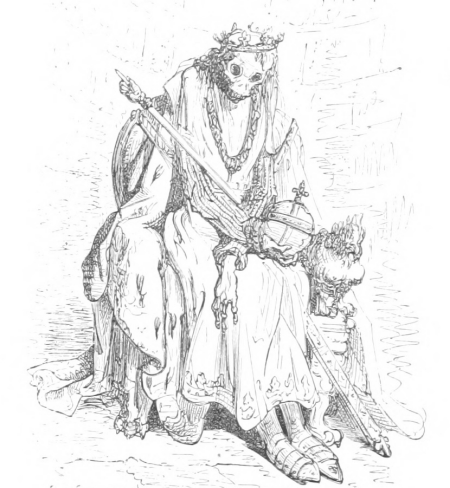
\includegraphics[scale=.5]{Lich}
  \end{center}



\newpage

\OCCULT[
  Name=Malison,
  Link=occultism-malison,
  Success=3+,
  Cost=See below
]

You can place one of the base {Curses}{table-curses}:

\mylist {
  \item on a person within [Cunning]km; 
  \item on an item; or 
  \item on your familiar.  
}

\mybullet{
    \item a \myital{random} Lesser Curse requires 3 [Cunning]
    \item a \myital{specific} Lesser Curse requires 5 [Cunning]
    \item a \myital{random} Greater Curse requires 7 [Cunning]
    \item a \myital{specific} Greater Curse requires 9 [Cunning]

}

You can break any of your own curses at will. Malisons will survive your death.  The cost to cast the curse is [Cunning]x10\AU


\OCCULT[
  Name=Unhallowed Earth,
  Link=occultism-unhallowed-earth,
  Success=2+ (plus see below),
  Cost=66\AU
]

You can either desecrate Hallowed Ground, or create Unhallowed Earth for the casting of rituals, somewhere within [Cunning]km of you.  You create / desecrate an area [Cunning]x2 meters in diameter.  If you're attempting to desecrate Hallowed Ground, the diameter must be equal to or exceed the area of the Hallowed Ground.  You must create a \mylink{Witch Mark}{occultism-witch-mark} that will be consumed during the ritual; this Witch Mark identifies the Unhallowed Earth as "belonging" to you.  Another Mystic knows the size of the Unhallowed Earth, but not necessarily who it belongs to.

Unhallowed Earth with your Witch Mark on it provides the following benefits:

\mybullet {
  \item no Mortals may enter Unhallowed Earth unless you accompany them
  \item you may immediately end a Markovian effect while standing on the Unhallowed Earth
  \item you may ignore the negative effect of a Failure when using your Mojo (that is, you may keep your Mojo die even if they roll a 1 or a 2) while standing on the Unhallowed Earth
  \item finally, no Sacraments may be performed on Unhallowed Earth
}

This ritual is the only one that does \mybold{not} require Unhallowed Earth to perform. 



\OCCULT[
  Name=Witch Mark,
  Link=occultism-witch-mark,
  Success=2,
  Cost=66\AG
]

A personal mark of power placed on any non-living item.  The mark itself is not magical, but requires the \mylink{Third Eye}{charm-third-eye} to see. Unless you've seen this Witch Mark before (if you knew them personally, for example), a Skill: Lore check is required to determine the owner of the Witch Mark.  Unhallowed Earth imbued with your Witch Mark follows the same rules (visible via the Third Eye, requires a Skill:Lore check to identify the owner).


